\documentclass[a4paper,11pt,dvipdfmx]{jsarticle}

\usepackage{url}

% 数式
\usepackage{amsmath,amsfonts}
\usepackage{bm}

% 画像
\usepackage[dvipdfmx]{graphicx}
\usepackage{framed}

% 図形
\usepackage{tikz}
\usetikzlibrary{shapes.geometric}
\usetikzlibrary {shapes.misc}

% ソースコード
\usepackage{listings,jlisting,color}
\lstset{
language={Python},
backgroundcolor={\color[gray]{.85}},
basicstyle={\ttfamily},
identifierstyle={\small},
commentstyle={\small \color[rgb]{0,0.5,0}},
keywordstyle={\small\bfseries \color[rgb]{0.5,0,0.5}},
ndkeywordstyle={\small},
stringstyle={\small\ttfamily \color[rgb]{0,0,1}},
frame={tb},
breaklines=true,
columns=[l]{fullflexible},
numbers=left,
xrightmargin=0zw,
xleftmargin=3zw,
numberstyle={\scriptsize},
stepnumber=1,
numbersep=1zw,
lineskip=-0.5ex,
}
\renewcommand{\lstlistingname}{ソースコード}

\begin{document}
\begin{titlepage}
\noindent
\vspace{6cm}
\begin{center}
\begin{LARGE}
通信システム実験2 待ち行列シミュレーション
\end{LARGE}
\end{center}
\vspace{6cm}
\begin{flushright}
信州大学工学部 \
電子情報システム工学科 \
\begin{description}
\setlength{\leftskip}{8.9cm}
\item[  実験日:] 2023/11/01
\item[ 実験場所:] W2棟101室
\item[  実験者:] 21T2166D 渡辺 大樹
\item[共同実験者:] 20T2062A 斎藤 創真
\item[      ] 21T2004H 朝日 純菜
\item[      ] 21T2033A 岡村 椋平
\item[      ] 21T2091J 徳竹 稜平
\item[      ] 21T2099D 中田 奏音
\end{description}
\end{flushright}
\end{titlepage}

\definecolor{shadecolor}{gray}{0.70}


\section{実験内容}
本実験ではネットワークにおけるパケット通信のレスポンスなどに用いられる
待ち行列理論をバスの運行シミュレーションを通してその理論の体験、理解を進める目的で行う。

実験1ではベルヌーイ過程を、実験2では指数分布をシミュレーション、理解し、これらを用いて実験3でバスの運行シミュレーションを行う。

\section{レポート課題}
以下にレポート課題の解答を示す。

\subsection*{レポート課題1.1}
確率変数$Z$の分布関数$F_Z(x)$を密度関数$f_Z(x)$で表すと
\begin{align}
    F_Z(x) = \int_{-\infty}^{\infty}f_Z(x)dx
\end{align}
となる。

\subsection*{レポート課題1.2}
到着確率の期待値が$\frac{\delta}{p}$となることを示す。

タイムスロットの間隔を$\delta$,各スロットでの到着確率を$p$としたときの到着間隔の期待値を求める。
到着間隔の確率変数を$Z$,確率を$P_Z(n)$とすると$n=1,2,3,\cdots$に対して確率$P_Z(n)$は
\begin{equation}
    \begin{split}
        P_Z(1) &= p \\
        P_Z(2) &= p(1-p) \\
        P_Z(3) &= P(1-p)^2 
    \end{split}
\end{equation}
となる。
期待値の式は確率変数とその時の確率を掛け合わせ、
\begin{align}
    E[Z] = \sum_{n=1}^{\infty}n \cdot \delta \cdot P_Z(n) 
\end{align}
となる。

この式に先ほどの確率$P_Z(n)$の一般化した式を代入することで
\begin{align}
    E[Z] = \delta p\sum_{n=1}^{\infty}n(1-p)^{n-1}
\end{align}
という式が得られる。

ここでシグマの中身を部分和として計算していく。
\begin{align}
    S_n = \sum_{k=1}^{n}k(1-p)^{k-1}
\end{align}
とする。
$S_n$に$(1-p)$を掛け算すると
\begin{align}
    (1-p)S_n = \sum_{k=1}^{n}k(1-p)^k
\end{align}
となる。
(5)から(6)を引き算すると
\begin{align}
    pS_n = \sum_{k=1}^{n+1}(1-p)^{k-1}
\end{align}
という式が得られる。この式は初項$1$公比$(1-p)$の等比数列の和となるため
公式を用いて計算すると
\begin{align}
    pS_n = \frac{1-(1-p)^n}{p}
\end{align}
となる。すなわち$S_n$は
\begin{align}
    S_n = \frac{1-(1-p)^n}{p^2}
\end{align}
となる。

$S_n$は部分和のためnについて極限をとることで
\begin{align}
    \sum_{n=1}^{\infty}n(1-p)^{n-1} = \frac{1}{p^2}
\end{align}
となる。これを(4)式に代入しなおすことで
\begin{align}
    E[Z] = \frac{\delta}{p}
\end{align}
が得られる。これにより題意は示された。

\subsection*{レポート課題1.3}
10面サイコロの0-9の目をすべて出すために必要なサイコロを振る回数の平均を求める。

サイコロの目をコンプリートする回数を計算することは上記課題1.2で行った
タイムスロットの到着間隔の期待値を考えることと同じで、k個目のサイコロの目がm回目で揃う確率は
$(\frac{k}{10})(1-\frac{k}{10})^{m-1}$となる。
これをmが無限大になるまで和を求めればよいためサイコロを振る回数の平均$E$は
\begin{align}
    E &= \sum_{k=1}^{10}\frac{1}{1-\frac{k}{10}}\\
      &= 10(\frac{1}{10}+\frac{2}{10}+\frac{3}{10}+\cdots+1)
\end{align}
となりしたがっておおよそ$E=29.28$という値が得られる。

\subsection{レポート課題2.1}
指数分布の密度関数が$f(x)=\lambda e^{-\lambda x}$であることを用いて
分布関数が$F(x)=1-e^{-\lambda x}$となることを示す。

密度関数を定義されるすべての$x$で積分することで分布関数が求まるので計算をすると
\begin{align}
    F(x) &= \int_{0}^{x}\lambda e^{-\lambda t}dt \\
         &= \left[-e^{-\lambda t}\right]_{0}^{x} \\
         &= 1 - e^{-\lambda x}
\end{align}
となり、よって題意は求まった。

\subsection{レポート課題2.2}
期待値は確率とそのときの値を掛け合わせたものび総和で求まる。指数分布は連続な確率関数なので
\begin{align}
    E[x] &= \int_{0}^{\infty}x(\lambda e^{-\lambda x})dx \\
         &= \left[xe^{-\lambda x}\right]_{0}^{\infty} - \lambda \int_{0}^{\infty} -\frac{1}{\lambda} e^{-\lambda x} dx \\
         &= -\frac{1}{\lambda} \left[e^{-\lambda x}\right]_{0}^{\infty} \\
         &= \frac{1}{\lambda}
\end{align}
と部分積分などを用いることで求まった。

\subsection{レポート課題2.3}
ここでは分布関数$F(x)=1-e^{-\lambda x}$の逆関数が$F^{-1}(x)=-\frac{1}{\lambda}\log(1-x)$
となることを示す。
\begin{align}
    y &= F(x) \\
      &= 1-e^{-\lambda x}
\end{align}
とする。$x$と$y$を入れ替えることで逆関数となる。入れ替えた後の関数を$y$について解いていく。
\begin{align}
    x &= 1 - e^{-\lambda y} \\
    e^{-\lambda y}  &= 1 - x \\
    -\lambda y &= \log(1-x) \\
    y &= -\frac{1}{\lambda}\log(1-x)
\end{align}
このように式を変形させることで示される。

\subsection{レポート課題3}
ランダムな到着とみなせる現象はレジの行列や自動販売機に支払われる硬貨などが挙げられる。

レジの行列はとてもポピュラーな例である。客がその任意のタイミングでレジ行列に並び、
レジでの会計が終わることでその処理が終了するため、ランダムな到着とみなせる。

自動販売機に支払われる硬貨も、その利用者が支払う際に自身が持つ任意の硬貨の組み合わせで
支払いを行うため、硬貨によるある程度の重み(例えば100円硬貨での支払いは多く、50円硬貨での支払いは少ない)がつく
と予想されるが、ランダムな到着とみなすことができる。

\section{実験}
以下に実験とその結果について示していく。

\subsection{実験1}
実験1では、間隔$\delta$により短く区切られた一つのタイムスロットでそれぞれ確率$p$の確率的施行
を行い、成功か失敗かを決める、ベルヌーイ過程を実験的に行う。

今回の実験では$\delta=1,p=0.1$として計算をおこなう。この施行ののち、到着まで
いくつのタイムスロットで失敗をしたのかの到着間隔をヒストグラムにまとめる。

実験にはPythonを用いて発生させた乱数が0.1より小さいときに成功、大きいと失敗とし失敗した場合はまた同じ
施行を繰り返させ、施行が失敗した回数を数えることでそれを到着間隔とした。

用いたコードは以下ソースコード\ref{bern}に示す。
\lstinputlisting[language=python,caption=Beenoulli.py, label=bern]{C:/Program_Code/Python/CSE2/Bernoulli.py}

このコードによって得られたヒストグラムを図\ref{berhist}に示す.
\begin{figure}[ht]
\centering
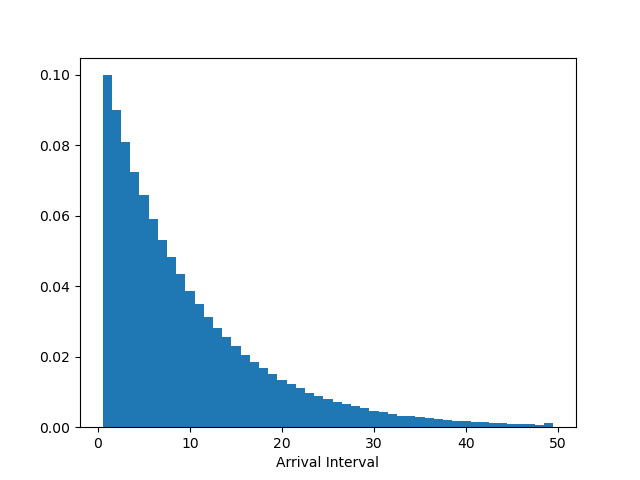
\includegraphics[width=80mm]{Bernoulli.png}
\caption{到着間隔の相対度数分布}
\label{berhist}
\end{figure}

この図\ref{berhist}が到着間隔の実験的な分布となる。

\subsection{実験2}
実験2では指数分布に従う乱数を実験的に発生させ、その累積相対度数のヒストグラムと平均値を
求め、指数分布の分布関数や期待値と比較していく。

一様乱数から任意の分布に従う確率変数を生成するには、今必要としている確率変数の分布関数を
$y=F(x)$,$[0,1)$の一様乱数を$U$としたとき
\begin{equation}
    X=F^{-1}(U)
\end{equation}
を計算すればよい。

レポート課題2.3で示した内容を用いれば、指数分布を一様乱数から生成するための式は
\begin{equation}
    X = -\frac{1}{\lambda}\log(1-U)
\end{equation}
となる。
この式から得られた乱数を統計的に処理して累積相対度数のグラフと平均値を取得する。

用いたコードは以下ソースコード\ref{expo}に示す。
\lstinputlisting[language=python,caption=Exporand.py, label=expo]{C:/Program_Code/Python/CSE2/Exporand.py}

このコードで得られたヒストグラムを図\ref{expohist}に示す。
\begin{figure}[ht]
\centering
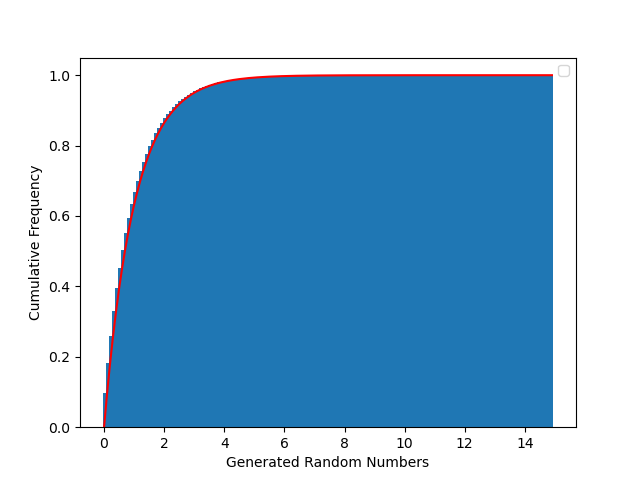
\includegraphics[width=80mm]{Exporand.png}
\caption{指数分布に従う乱数の累積相対度数と指数分布の分布関数}
\label{expohist}
\end{figure}

図\ref{expohist}では青色のヒストグラムが実験で発生させた乱数の累積グラフ、
赤色のグラフが指数分布の分布関数になっている。どちらともパラメータ$\lambda$は$1$で計算している。
ここからわかるように、ほとんど一致したグラフを生成できていることがわかる。

またこの施行で得られた平均値は0.999425708871489となった。
期待値は$\frac{1}{\lambda}$であることから$\lambda=1$であるとき期待値も$1$となるため、
そこそこの精度で一致していることが読み取れる。

\subsection{実験3 - 結果}
実験3ではパラメータ$\lambda_1$のポアソン過程に従って到着するバスに、
パラメータ$\lambda_2$のポアソン過程に従って到着する乗客が乗るようなバスの運行をシミュレートしていく。条件として到着し、
バスが来るまで待っている乗客はすべて到着したバスに乗るものとしてシミュレートする。

またパラメータ$\lambda_1,\lambda_2$はその都度適宜変更していく。

実験ではソースコード\ref{bus}を用いた。
\lstinputlisting[language=python,caption=Buses.py, label=bus]{C:/Program_Code/Python/CSE2/Buses.py}

先にソースコード\ref{bus}を実行して得られた乗客者数、同乗者数、乗客の待ち時間の平均を
いくつかの$\lambda$で求めた結果を表\ref{result}にして示しておく。
\begin{table}[ht]
    \centering
    \caption{実験3で得られた平均値}
    \begin{tabular}{|r|r|r|r|r|} \hline
        $\lambda_1$ & $\lambda_2$ & 乗客者数平均 & 同乗者数平均 & 待ち時間平均 \\ \hline
        1 & 5  & 5.00864 & 10.97850 & 1.00119 \\ \hline
        2 & 5  & 2.49612 & 5.99988  & 0.49941 \\ \hline
        1 & 10 & 9.99268 & 20.96280 & 0.99802 \\ \hline
        2 & 10 & 5.01614 & 11.05486 & 0.50255 \\ \hline
    \end{tabular}
    \label{result}
\end{table}

\subsubsection{実験3.1}
実験3.1ではバスの平均乗客者数とその乗客者数の分布について調べていく。

ソースコード\ref{bus}上では、平均乗客者数と乗客者数の分布を実験的に調べるためにwhile文を用いた。
while文では脱出条件として、次に来るバスについて、それまでのバスの到着間隔の累積和よりもこれまで来た乗客の到着間隔の累積和
が大きくなる時に脱出する、すなわちバスが次に来た段階で乗客のカウントをリセットさせている。
逆に脱出条件に達していないときはバスの乗客のカウントを一つ増やし、次に来る乗客の到着間隔を新たに乱数で生成している。

この乗客者数のカウントを配列にそれぞれ保存していき、その配列の頻度分析をすることで乗客者数の分布を、
平均を求めることで乗客者数の平均をそれぞれ求めていく。

ソースコード\ref{bus}で得られた乗客者数の相対度数分布のグラフを以下図\ref{3.1.1},\ref{3.1.2}に示す。
\begin{figure}[h]
    \begin{minipage}[b]{0.48\columnwidth}
      \centering
      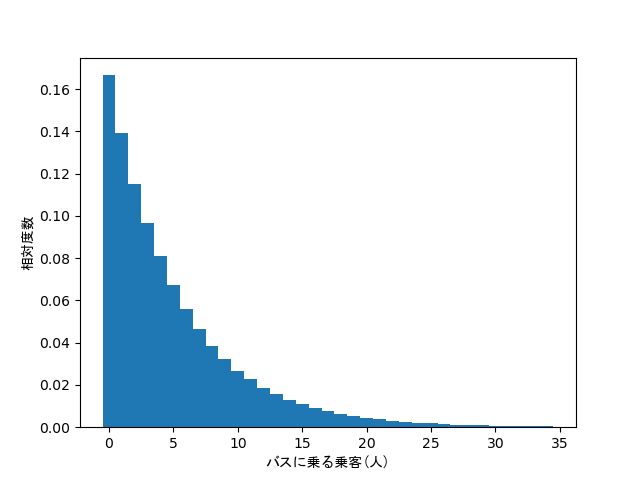
\includegraphics[width=\columnwidth]{C:/Program_Code/LaTeX/CSE2/Bus_cus_1_5.png}
      \caption{$\lambda_1=1,\lambda_2=5$のときの乗客者数ヒストグラム}
      \label{3.1.1}
    \end{minipage}
    \hspace{0.04\columnwidth} 
    \begin{minipage}[b]{0.48\columnwidth}
      \centering
      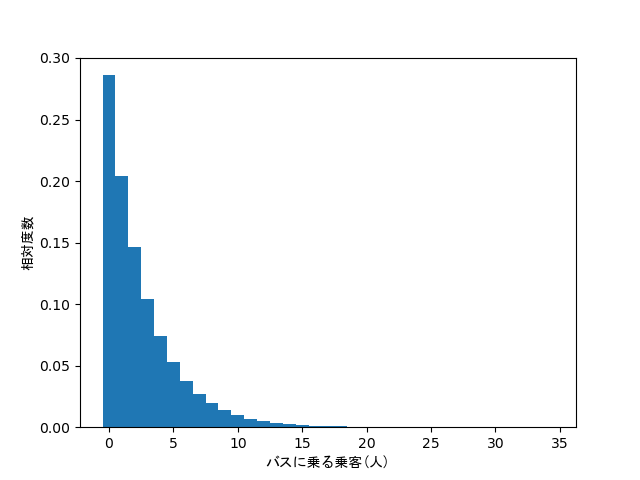
\includegraphics[width=\columnwidth]{C:/Program_Code/LaTeX/CSE2/Bus_cus_2_5.png}
      \caption{$\lambda_1=2,\lambda_2=5$のときの乗客者数ヒストグラム}
      \label{3.1.2}
    \end{minipage}
\end{figure}

乗客者数の平均は表\ref{result}に示してあるが、再度乗客者数の平均だけ表\ref{result_1}に示す。
\begin{table}[ht]
    \centering
    \caption{実験3で得られた乗客者数平均値と$\frac{\lambda_2}{\lambda_1}$の値}
    \begin{tabular}{|r|r|r|r|} \hline
        $\lambda_1$ & $\lambda_2$ & 乗客者数平均 & $\frac{\lambda_2}{\lambda_1}$  \\ \hline
        1 & 5  & 5.00864 & 5   \\ \hline
        2 & 5  & 2.49612 & 2.5 \\ \hline
        1 & 10 & 9.99268 & 10  \\ \hline
        2 & 10 & 5.01614 & 5   \\ \hline
    \end{tabular}
    \label{result_1}
\end{table}

図\ref{3.1.1},\ref{3.1.2}を見ると指数分布のような度数分布として出力されている。
表\ref{result_1}を見ると乗客者数平均と$\lambda$にある関係が見える。

小数誤差を考慮し整理すると、乗客者数平均を$C_{ave}$としたとき
\begin{equation}
    C_{ave} = \frac{\lambda_2}{\lambda_1}
\end{equation}
となることが考えられる。

また前述したように図\ref{3.1.1},\ref{3.1.2}では指数分布のような度数分布になったが実際に期待値が
$C_{ave}$となるような指数分布を図\ref{3.1.1}に重ねると図\ref{3.1.3}のようになった。
\begin{figure}[h]
    \centering
    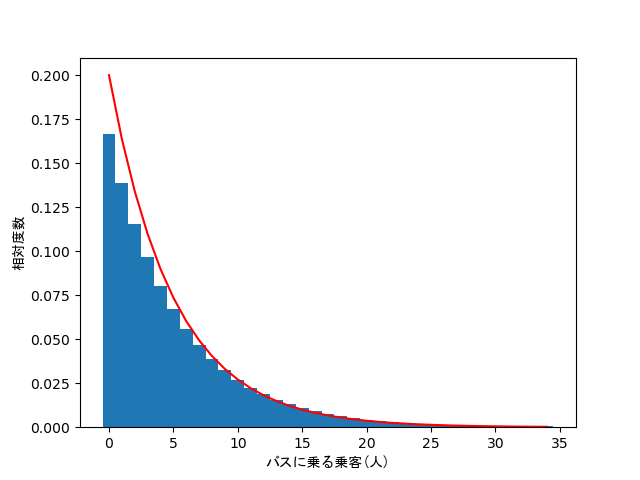
\includegraphics[width=80mm]{./Bus_cus_2_10_exp.png}
    \caption{図\ref{3.1.1}に$\frac{1}{C_{ave}}$がパラメータとなる指数分布を重ねたヒストグラム}
    \label{3.1.3}
\end{figure}

この図\ref{3.1.3}を見ると赤線で示される期待値が$C_{ave}$となる密度関数と、
実験で得た度数分布がかなり類似した分布になっていることが分かる。
この分布の類似は$\lambda$を別の値に変えても確認された。

\subsubsection{実験3.2}
実験3.2ではバスの中の乗客から見た混み具合、すなわち乗客から見たバスの同乗者数の分布とその平均値を求めていく。

ソースコード\ref{bus}内では、同乗者数というものを、バスの乗客全員から見た、そのバスに乗っている、自分を含めた同乗者をすべてカウントする
と解釈して実装した。
すなわち同乗者数は乗客者数の2乗でカウントされる。前実験で用いた乗客者数のリストをPythonのリスト内包表記を二重で用いることで
配列のすべての要素一つ一つの要素数をその要素の2乗に増やしている。この配列をnumpyに付属する関数で解析して度数分布を、
乗客者数で割ることで乗客から見た同乗者数の平均を求めている。

ソースコード\ref{bus}を実行することで得られた同乗者数の相対度数分布のグラフを以下図\ref{3.2.1},\ref{3.2.2}に示す。
\begin{figure}[ht]
    \begin{minipage}[b]{0.48\columnwidth}
      \centering
      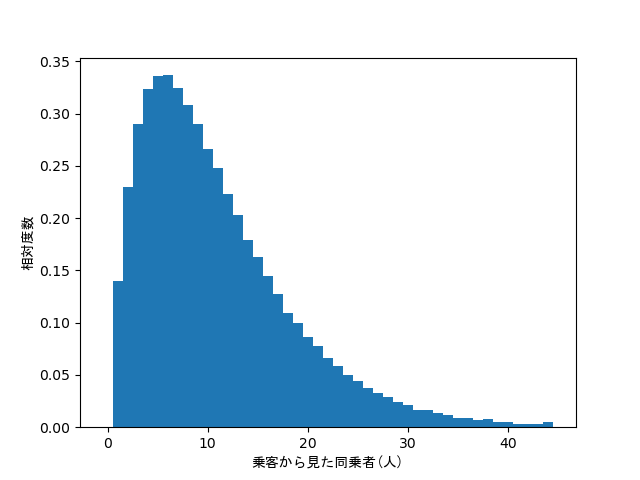
\includegraphics[width=\columnwidth]{C:/Program_Code/LaTeX/CSE2/Bus_pass_1_5.png}
      \caption{$\lambda_1=1,\lambda_2=5$のときの同乗者数ヒストグラム}
      \label{3.2.1}
    \end{minipage}
    \hspace{0.04\columnwidth} 
    \begin{minipage}[b]{0.48\columnwidth}
      \centering
      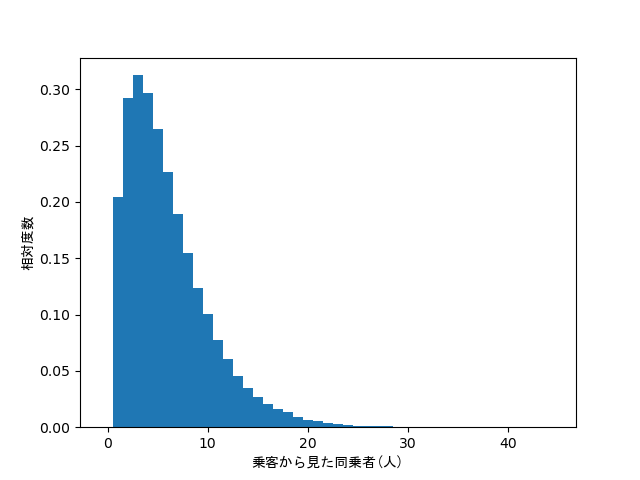
\includegraphics[width=\columnwidth]{C:/Program_Code/LaTeX/CSE2/Bus_pass_2_5.png}
      \caption{$\lambda_1=2,\lambda_2=5$のときの同乗者数ヒストグラム}
      \label{3.2.2}
    \end{minipage}
\end{figure}

同乗者数の平均も表\ref{result}に示してあるが、再度同乗者数の平均を表\ref{result_2}に示す。
\begin{table}[ht]
    \centering
    \caption{実験3で得られた同乗者数平均値と$2\frac{\lambda_2}{\lambda_1}+1$の値}
    \begin{tabular}{|r|r|r|r|} \hline
        $\lambda_1$ & $\lambda_2$ & 同乗者数平均 & $2\frac{\lambda_2}{\lambda_1}+1$  \\ \hline
        1 & 5  & 10.97850 & 11 \\ \hline
        2 & 5  & 5.99988  & 6  \\ \hline
        1 & 10 & 20.96280 & 21 \\ \hline
        2 & 10 & 11.05486 & 11 \\ \hline
    \end{tabular}
    \label{result_2}
\end{table}

図\ref{3.2.1},\ref{3.2.2}を見ると$\chi$二乗分布のようなヒストグラムに見えるが、
実際、一様分布ではない乱数の二乗和の分布となるので$\chi$二乗分布の密度関数に近づくことも考えられる。ただ$\chi$二乗分布ではない。

表\ref{result_2}から同乗者数の平均と$\lambda$の値の関係を考えてみると同乗者数の平均値を$P_{ave}$とすると
\begin{equation}
    P_{ave} = 2\frac{\lambda_2}{\lambda_1}+1
\end{equation}
となることが考えられる。実際にこの式に$\lambda$を代入して計算した値を表\ref{result_2}に示している。

\subsubsection{実験3.3}
実験3.3ではバスの乗客がバス停に到着してからバスが着くまでに待つ時間の分布とその平均値を求めていく。

ソースコード\ref{bus}内では、乗客が乗るバスが到着した時間からその乗客が到着した時間を引くことで待ち時間を求めている。
この待ち時間を配列に追加していくことで、その配列を解析して度数分布を、その配列の平均値をとることで待ち時間の平均を求めている。

ソースコード\ref{bus}を実行することで得られた同乗者数の相対度数分布のグラフを以下図\ref{3.3.1},\ref{3.3.2}に示す。
\begin{figure}[ht]
    \begin{minipage}[b]{0.48\columnwidth}
      \centering
      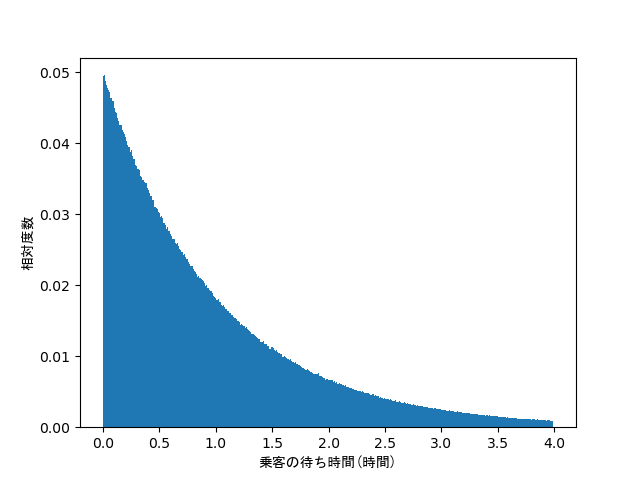
\includegraphics[width=\columnwidth]{C:/Program_Code/LaTeX/CSE2/Bus_time_1_5.png}
      \caption{$\lambda_1=1,\lambda_2=5$のときの待ち時間ヒストグラム}
      \label{3.3.1}
    \end{minipage}
    \hspace{0.04\columnwidth} 
    \begin{minipage}[b]{0.48\columnwidth}
      \centering
      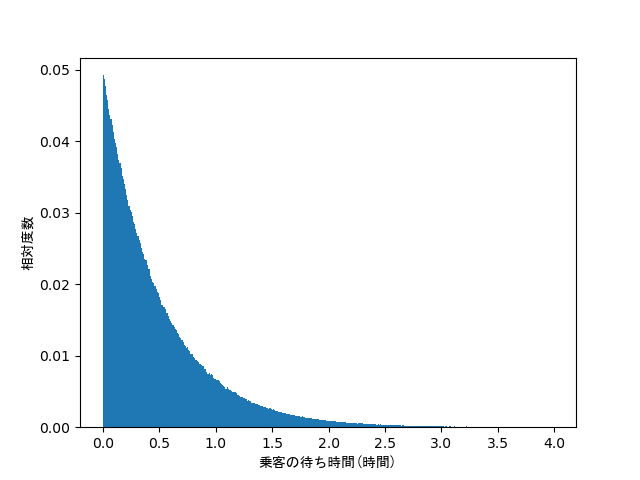
\includegraphics[width=\columnwidth]{C:/Program_Code/LaTeX/CSE2/Bus_time_2_5.png}
      \caption{$\lambda_1=2,\lambda_2=5$のときの待ち時間ヒストグラム}
      \label{3.3.2}
    \end{minipage}
\end{figure}

同乗者数の平均も表\ref{result}に示してあるが、再度乗客の待ち時間の平均を表\ref{result_3}に示す。
\begin{table}[ht]
    \centering
    \caption{実験3で得られた乗客の待ち時間の平均値と$\frac{1}{\lambda_1}$の値}
    \begin{tabular}{|r|r|r|r|} \hline
        $\lambda_1$ & $\lambda_2$ & 乗客の待ち時間の平均 & $\frac{\lambda_2}{\lambda_1}$  \\ \hline
        1 & 5  & 1.00119 & 1   \\ \hline
        2 & 5  & 0.49941 & 0.5 \\ \hline
        1 & 10 & 0.99802 & 1   \\ \hline
        2 & 10 & 0.50255 & 0.5 \\ \hline
    \end{tabular}
    \label{result_3}
\end{table}

図\ref{3.3.1},\ref{3.3.2}を見ると指数分布のようなヒストグラムに見える。

表\ref{result_3}から乗客の待ち時間の平均と$\lambda$の値の関係を考えてみると乗客の待ち時間の平均値を$T_{ave}$とすると
\begin{equation}
    T_{ave} = \frac{1}{\lambda_1}
\end{equation}
となることが考えられる。実際にこの式に$\lambda$を代入して計算した値を表\ref{result_2}に示している。

\subsection{実験3 - 考察}
以下で実験3の結果について考察していく。
\subsubsection{考察1}
考察1ではバスの平均乗客者数と乗客の平均同乗者数を比較し、関係を考える。先の実験3.1,3.2においてそれぞれの平均値の理論式を
\begin{align}
    C_{ave} &= \frac{\lambda_2}{\lambda_1} \\
    P_{ave} &= 2\frac{\lambda_2}{\lambda_1}+1
\end{align}
と推定した。

この二式より関係は
\begin{equation}
    P_{ave} = 2C_{ave}+1
\end{equation}
とすることができる。
この(34)式がどのように導出されているのかについて考察していく。
ただここでは$C_{ave}$の理論的な導出は易しいものではないことが予想されるので経験則に基づく式にはなるがこのまま用いる。

この導出を考える前に$P_{ave}$をどのように求めたかに立ち返って考える。実験では乗客者数の二乗和を乗客者数で割った値として計算した。
これはすなわち乗客者数をある密度関数$f(x)$に従う確率変数$X$としたとき、$+1$の項を無視すれば
\begin{equation}
    P_{ave} = \frac{\sum X^2}{\sum X}
\end{equation}
を計算していることになる。

ここでこの分数をバスの台数となる$n$で分母分子割ると
\begin{equation}
    P_{ave} = \frac{\frac{\sum X^2}{n}}{\frac{\sum X}{n}}
\end{equation}
となる。ここでこの分母$\frac{\sum X}{n}$は乗客者数の総和をバスの台数で割ったもの、すなわちバス一台あたりの乗客者数$C_{ave}$
と同じになる。
ということで式は
\begin{equation}
    P_{ave} = \frac{\frac{\sum X^2}{n}}{C_{ave}}
\end{equation}
と変形できる。

ここで分子に注目していく。先の実験3.1で図\ref{3.1.3}のように、乗客者数の分布は平均値が$C_{ave}$となる指数分布によく似ている
という指摘をした。これを参考に$X$が実際に平均値が$C_{ave}$となる指数分布に従う確率変数だと仮定すると式(37)の分子は
指数分布の確率変数の二乗平均となり、これは実際に計算が可能である。
詳細な計算方法は省く\cite{exp}が指数分布における二乗平均は平均値が$E[x]$のとき$2E[x]^2$となることが知られている。
これをそのまま式(37)に代入することで
\begin{align}
    P_{ave} &= \frac{2C_{ave}^2}{C_{ave}} \\
            &= 2C_{ave}
\end{align}
と計算でき、$+1$の項を無視してしまっているがおよそ関係が導出できたのではないかとおもう。

\subsubsection{考察2}
考察2では乗客の平均待ち時間とバスの平均間隔の関係について考察していく。

バスの平均間隔はパラメータ$\lambda_1$の指数分布を用いてバスの到着間隔を求めているため、理論値として$\frac{1}{\lambda_1}$となる。
乗客の平均待ち時間は実験3.3の結果より類推して経験則的に$\frac{1}{\lambda_1}$であると予測した。

この二つの式は同じ式となっていることが分かる。
この二式がどのように同じになるのかは単純で、$\lambda_2$が関係してこない事象のため乗客の到着間隔を単位時間に固定して考えると、
レート$\lambda_1$のポアソン過程に従うバスの到着から待ち時間を考えることはバスの到着間隔を求めていることと相違ないことが分かる。

したがってこの二式が同じものとなることが分かる。

\begin{thebibliography}{99}
    \bibitem{exp} 指数分布の期待値・分散の導出(証明) | AVILEN AI Trend \url{https://ai-trend.jp/basic-study/exponential-distribution/e-parameter-derivasion/} 2023/11/23 閲覧
\end{thebibliography}

\end{document}